\section{Methods}

We propose an optimization procedure that incrementally minimizes mesh vertex noises using differentiable rendering. 
Suppose we have vertices $V=\{V_i\in\mathbb{R}^3\}=\{V_0...V_n\}$ within input mesh $\mathcal{M}$ which is fused from input color $\mathcal{C}$ and depth $\mathcal{D}$ with intrinsic $K$ such that $\mathcal{M}=K^{-1}\left(\mathcal{C}\oplus \mathcal{D}\right)$. 
Here, $\oplus$ denotes image registration operator.
We pre-computed $\mathcal{M}$ from popular off-line SLAM framework \cite{zhou2018open3d} with voxel size 2cm.
We define deformed vertices $V_d$, which has same shape as $V$ initialized with zero values i.e., $V_d=\{\mathbf{0}_0,...,\mathbf{0}_n\}$. 
For every iteration, $V_d$ is optimized so that resulting vertices $V_o=V+V_d$ approximate noise-free geometry which looks perceptually similar with $\mathcal{C}$. 
\PJ{Emphasize minimizing difference between GT color and rendered color.}
The main problem is how to find common geometric representations between $\mathcal{C}$ and $C$ to figure out which region is to be optimized (i.e., noisy).

\paragraph{Assumptions}
Our goal is to minimize vertex noise of TSDF mesh $\mathcal{M}$ fused from a single pair of indoor RGB-D images $\mathcal{C}\oplus \mathcal{D}$. Given this scenario, we assume that we known camera intrinsic $K$ and extrinsic $T=I\in\mathbb{R}^{4*4}$. 
We will also consider the captured real scene is Lambertian, as all SLAM datasets are generated under Lambertian-dominant assumption to guarantee accurate camera pose estimate, unless additional consideration of non-Lambertian scene is introduced. \PJ{TODO: refer [Whelan, 2018]}
We additionally constrain that there are no strong texture changes under geometrically close, flat surfaces. 

\subsection{Interpreting Perceptually Noise-free Geometry from Color Image}
\PJ{Too verbose! TODO: add proof}
In this section, we formally describe our intuition that enables input color image treated as noise-free geometric clue.

Let us consider $\mathcal{C}$ as a result from perfect renderer which is capable of tracing full light transport without any noise and outlier, given unknown lighting conditions and noise-free geometry. 
Based on Light Transport Equation(LTE) representation with respect to path integral form \cite{veach1998robust}, we represent $\mathcal{C}$ as a set of solution of LTE for each pixel:

\begin{align}
    \mathcal{C} & = \bigcup_i^W \bigcup_j^H L_{i,j}\left(K^{-1}\cdot x\rightarrow p_0\right) \nonumber \\
    & = \bigcup_i^W \bigcup_j^H L_{i,j}\left(p_1'\rightarrow p_0\right),
\end{align}
where $L_{i,j}$ is total radiance at a pixel, and $p_1'=K^{-1}\cdot x$ is hitpoint of $L_{i,j}$.

To intuitively exploit relationship between $\mathcal{C}$ and noise-free hitpoint $x_{i,j}$, we expand radiance sum over path:
\begin{align}
    L_{i,j}\left(p_1'\rightarrow p_0\right)& = [\mathit{P\left(\bar{\mathrm{p}}_1\right)}+\mathit{P\left(\bar{\mathrm{p}}_2\right)}]+[\sum_{n=3}^\infty \mathit{P}\left(\bar{\mathrm{p}}_n\right)], 
    \label{LTE_path_integral}
\end{align}

where $\bar{\mathrm{p}}_n=\mathrm{p}_0\mathrm{p}_1...\mathrm{p}_n$ is path segment with $n+1$ vertices. We examine emitted radiance i.e., Albedo and direct lighting term in (Eqn. \ref{LTE_path_integral}):

\begin{align}
    \mathit{P\left(\bar{\mathrm{p}}_1\right)}+\mathit{P\left(\bar{\mathrm{p}}_2\right)}=\int_A & f\left(p_2\rightarrow p_1\rightarrow p_0\right)\cdot L_{e (i,j)}\left(p_2\rightarrow p_1\right)\cdot \nonumber \\
    & V\left(p_1 \leftrightarrow p_2\right) \cdot dA\left(p_2\right)
\end{align}


% Our key observation is strong radiance change within color images $\mathcal{C}$ and $C$, is only occurred from strong geometric displacements around a corresponding pixel. 
% This is possible since we made two assumptions: Lambertian-dominant scene, and no strong texture changes under flat surface. 
% Consider $\mathcal{C}$ is generated from perfect renderer 
% which are capable of tracing full light transport, under perfect geometries. 
% Although we cannot know which lighting conditions are used to render $\mathcal{C}$, 
% however, at least we know the lighting is somehow applied to 
% perfect geometries since $\mathcal{C}$ is rendered, as well as we are able to perceive geometric information by just observing $\mathcal{C}$. 
% Using the fact that $\mathcal{C}$ is a discretization of continuous radiance function, 
% we can intuitively notice that changing lighting condition 
% never affects to local radiance change (unless the light is very close to the surface).
% From this intuition, we can render $\mathcal{M}$ over virtually placed light source(s). 
% If $\mathcal{M}$ is noise-free enough, there would be no highlighted pixel in its rendering $C$. 
% However, due to the fact that $C$ is rendered with $\mathcal{C}$ from noisy measurement $\mathcal{D}$, 
% there exist a set of saturated pixel, which are actually not saturated within $\mathcal{C}$. 
% Based on this observation, we decided to minimize gap between saturated pixels in $C$ and unsaturated i.e., noise-free pixels in $\mathcal{C}$. 
% In order to do this, it is required to detect noise-free pixels in $\mathcal{C}$, as well as noisy pixels in $C$, 
% and set the difference as loss function so that our differentiable renderer properly minimizes gap.

\subsection{Detecting Geometric Information given Color Image and Its Rendering}
We simply detect noise-free surfaces within $\mathcal{C}$ by applying Scharr gradient kernel. 
Under the assumption that the scene is Lambertian-dominant and there is no sudden strong texture changes around the same surface, 
we found that this is enough to capture which region is smooth in terms of radiance (i.e., geometrically noise-free). 
In order to ensure robustness on strong texture changes 
one may combine with gradient from $\mathcal{D}$, but for this report we only experimented with gradients from $\mathcal{C}$. Specifically, Scharr kernel for each axis over an image is defined as
\begin{equation}
    \label{eqn:01}
    G_x=\begin{pmatrix}
        -3 & 0 & 3\\
        -10 & 0 & 10\\
        -3 & 0 & 3
    \end{pmatrix}, 
    G_y=\begin{pmatrix}
        -3 & -10 & -3\\
        0 & 0 & 0\\
        3 & 10 & 3
    \end{pmatrix}
\end{equation}
, and our detected geometric changes over Ground Truth color image $\widetilde{G}_\mathcal{C}$ is a Scharr gradient of $I_\mathcal{C}$ i.e., the intensity image from $\mathcal{C}$. 
Since resulting gradient on some pixels have negative value of identical magnitude to positive values of neighboring pixel, we take its absolute value
\begin{equation}
    \label{eqn:02}
    \widetilde{G}_\mathcal{C}=\frac{1}{2}\left(|G_x\left(I_\mathcal{C}\right)|+|G_y\left(I_\mathcal{C}\right)|\right)
\end{equation}
In order to detect noisy vertices over TSDF mesh, we propose Lightweight map to determine which vertex has stronger noise compare to $\widetilde{G}_\mathcal{C}$. 
Lightweight map $I\textsubscript{lw}$ is an image taken from identical camera setup to $\mathcal{C}$, but holds how much a pixel corresponds to a hitpoint is affected by virtual light at a shading stage.
$I\textsubscript{lw}$ is defined as
\begin{equation}
    I\textsubscript{lw}=\{I\textsubscript{lw,i}\in\mathbb{R}\textsuperscript{\textit{W}*\textit{H}}\}, I\textsubscript{lw,i}=\frac{\left(x_i-p_0\right)\cdot n_i}{d\left(x_i,p_0\right)+\epsilon}, 
\end{equation}
where $x_i$, $n_i$ is world position and normal of hitpoint with pixel index \textit{i}, respectively. 
$p_0$ is position of virtual light, and $d\left(x_i, p_0\right)$ is Euclidean distance between hitpoint and light position.
We obtain changing amount of each lightweight value $\widetilde{G}\textsubscript{lw}$ by applying Scharr kernel over $\textit{I}\textsubscript{lw}$, similar with $\widetilde{G}_\mathcal{C}$.
\begin{equation}
    \widetilde{G}_\textsubscript{lw}=\frac{1}{2}\left(|G_x\left(I\textsubscript{lw}\right)|+|G_y\left(I\textsubscript{lw}\right)|\right)
\end{equation}
We found that using geometric normal to calculate lightweight map saturate pixels around noisy vertices rather than shading normal, 
as shading normal smooths normal of each hit-point using neighboring vertex normal and its barycentric coordinates. 
In detail, pixels within same face have similar lightweight values 
since they are both geometrically close to each other, and they share same normal. 
Pixels that are geometrically close, but within different faces 
are highly likely to have similar values if two faces have near identical normal values. 
This is the case when two faces are considered as ‘flat’ to each other, 
meaning that shared vertices have no noise. 
As the vertex have bigger noise, the gap or normal between sharing two faces also gets bigger. 
This brings pixels in $G\textsubscript{lw}$ have large value where there is significant normal difference, meaning that the region has noisy vertex. 
Note that larger $G\textsubscript{lw}$ at a pixel means that the pixel has higher noise, therefore differentiable renderer can optimize the region more aggressively. 
This is illustrated in Figure 3.
We observed that the intensity image of rendered scene with virtual light $I_C$ serves similar role with $I\textsubscript{lw}$ as they properly reflect strong gradients around deviating normal.
Therefore, we note that for all results we used $I_C$ instead of $I\textsubscript{lw}$.
\begin{figure*}
    \centering
    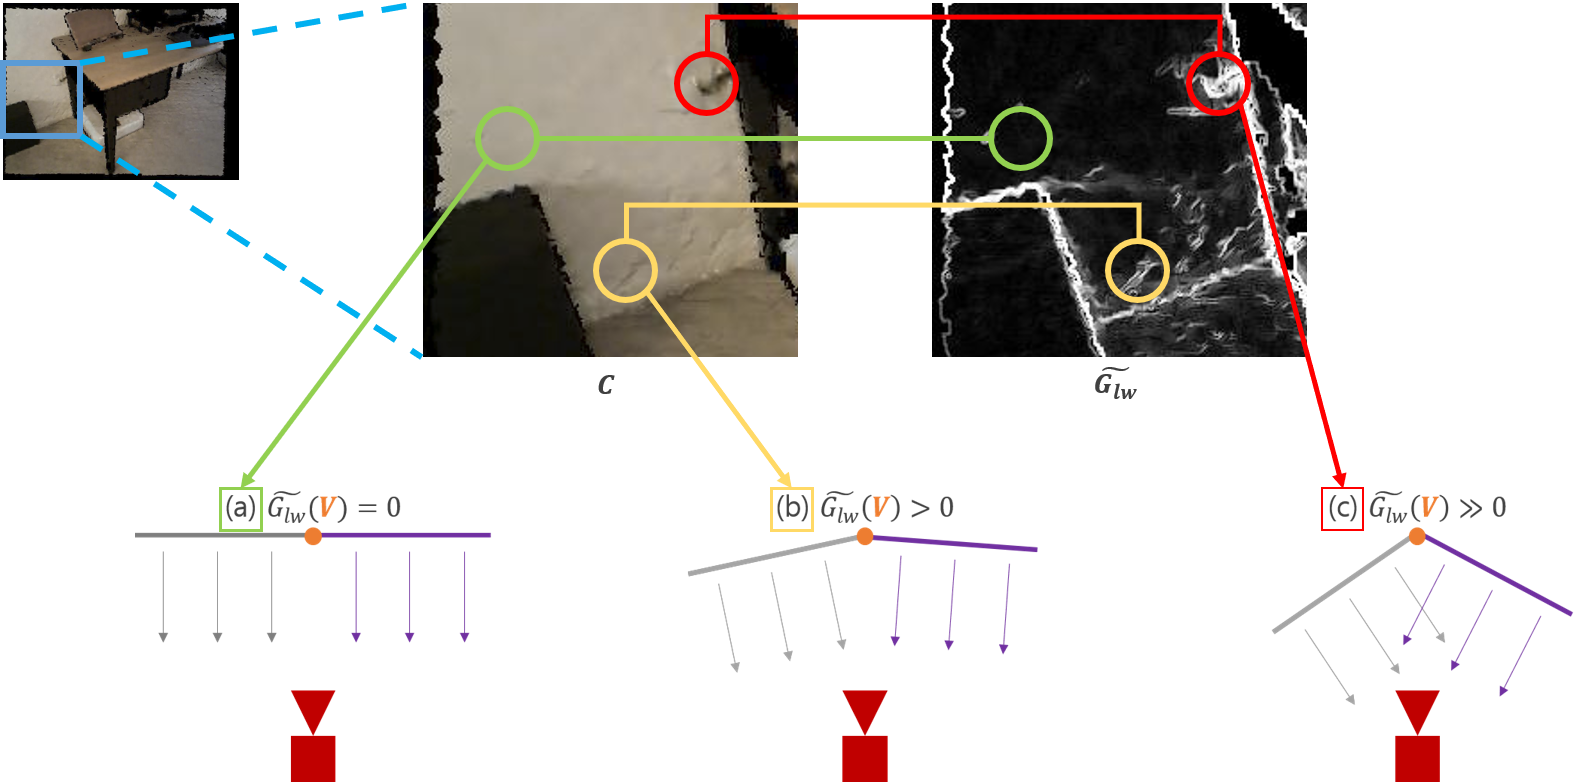
\includegraphics[width=\textwidth]{figures/3_method_relationship_gradient_lightweight_and_noise_full_tone_changed.png}
    \caption{Relationship between $G\textsubscript{lw}$ and actual noise of vertex $\textcolor{Orange}{V}$. We manually selected three pixels, where each have different magnitude of $G\textsubscript{lw}$. We also illustrated 1D example of the relationship. \textbf{\textcolor
    {Gray}{Gray}} and \textbf{\textcolor{Purple}{Purple}} lines and arrows indicate each face and its geometric normal. \textbf{\textcolor{LimeGreen}{(a)}} $\textcolor{Orange}{V}$ is considered as noise-free since $G\textsubscript{lw}$ is evaluated as zero, meaning adjacent faces have identical normal value. \textbf{\textcolor{Dandelion}{(b)}} $G\textsubscript{lw}$ is increased as two faces have inconsistent normal. \textbf{\textcolor{Red}{(c)}} as $G\textsubscript{lw}$ gets bigger, $\textcolor{Orange}{V}$ is considered as highly-noisy vertex. From these examples, we can say that $G\textsubscript{lw}$ precisely indicates where noisy pixels exist.}
    \label{fig:relationship_gradient_lightweight_and_noise}
\end{figure*}

\subsection{Optimization using Differentiable Rendering}
We define lightweight loss to minimize the difference between noise-free geometric information $\widetilde{G}_\mathcal{C}$ and noise-detected rendered image $\widetilde{G}_C$. We found that there is gradient value range inconsistency between $\widetilde{G}_\mathcal{C}$ and $\widetilde{G}_C$, as they are derived from different type of image i.e., color and geometry, respectively. We applied hyperbolic tangent kernel to each gradient image to ensure that both images have normalized value range, and we observed that this helped optimizer to find optimal without failure. Finally, we replace our target GT image from $\mathcal{C}$ to $\mathcal{C}\oplus\mathcal{D}$, as $\mathcal{M}$ follows holes where pixels in $\mathcal{D}$ have zero value. Our final geometric gradients are:
\begin{equation}
    G_\mathcal{C}=\tanh\left(\widetilde{G}_{\mathcal{C}\oplus\mathcal{D}}\right),
    G_{lw}=\tanh\left(\widetilde{G}_{lw}\right), 
\end{equation}
where $\tanh\left(x\right)=\frac{e^x-e^{-x}}{e^x+e^{-x}}$. Our optimizer minimizes lightweight loss representing geometric difference, while penalizing vertices not to evolve too far from its initial position:
\begin{gather}
    \mathcal{L}=w_{lw}\cdot L_{lw}+w_{pos}\cdot L_{pos}, \\
    L_{lw}=\left|\left|G_\mathcal{C}-G_C\right|\right|^2_2, \\
    L_{pos}=\left|\left|V-\left(V_o\right)\right|\right|^2_2=\left|\left|V_d\right|\right|^2_2
\end{gather}
For all results, we used $w_{lw}=0.01$ and $w_{pos}=1.0$. Fig. 4 visualizes optimization procedure.
\begin{figure}
    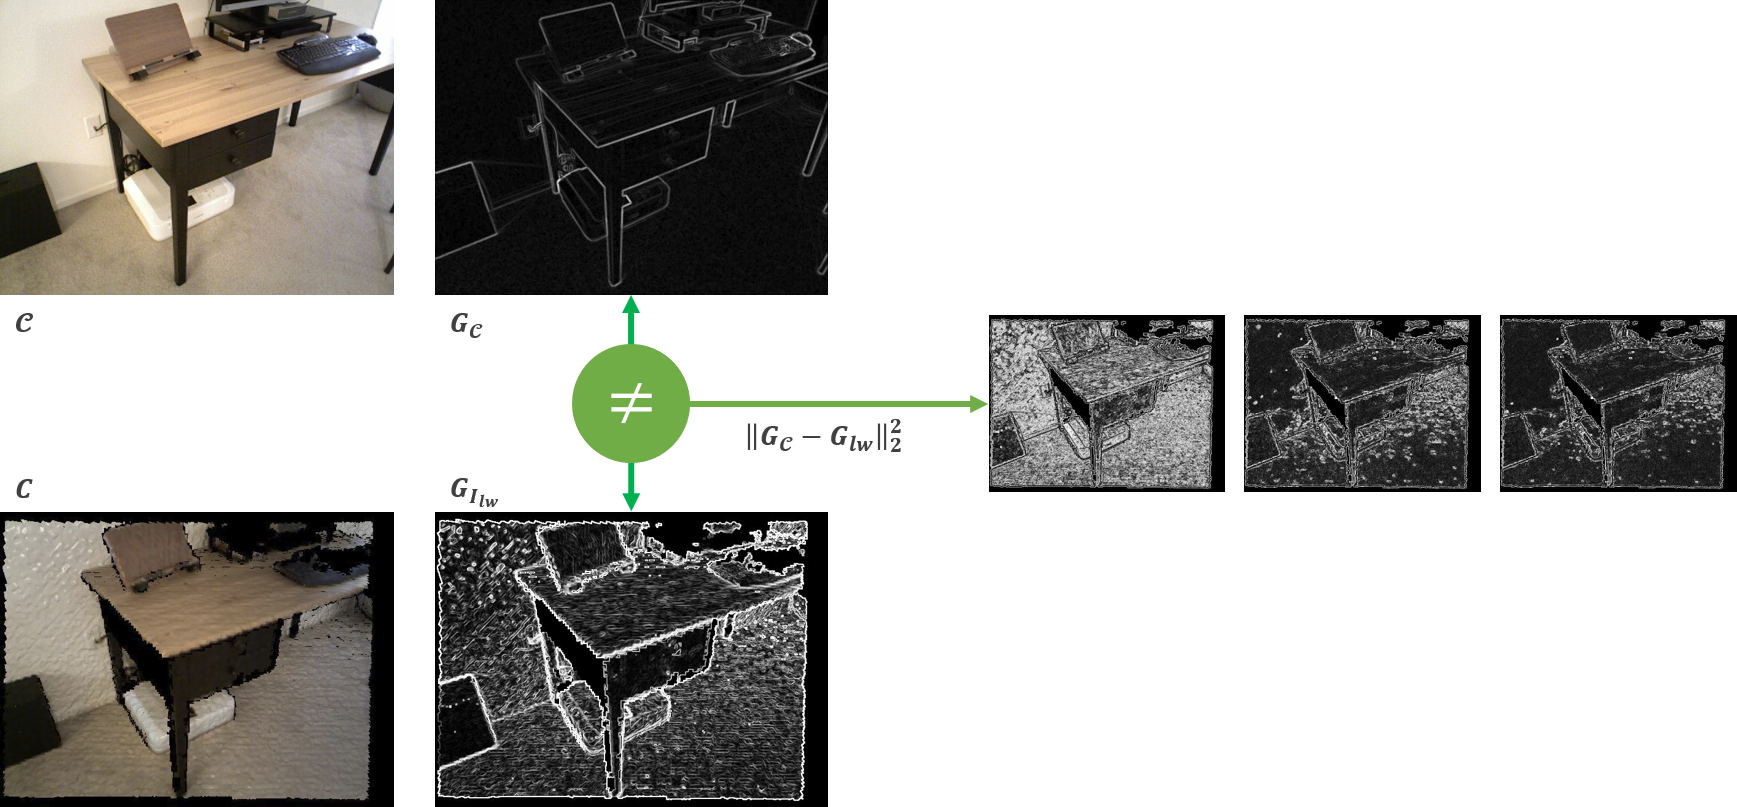
\includegraphics[width=\columnwidth]{figures/3_method_optimization.png}
    \caption{Optimization procedure of our differentiable rendering. From generated target noise-free geometric clue $G_\mathcal{C}$ and input noisy geometric clue $G_{lw}$, we minimize $L_2$ distance between two clues. Note that we additionally penalize aggressive vertex evolve, however it is skipped in the figure.}
    \label{fig:optimization}
\end{figure}